\documentclass[10pt]{article}

% Suppress volatile pdfTeX metadata.  The build driver also fixes
% SOURCE_DATE_EPOCH so included Matplotlib PDFs receive stable timestamps.
\ifdefined\pdfinfoomitdate\pdfinfoomitdate=1\fi
\ifdefined\pdftrailerid\pdftrailerid{}\fi
\ifdefined\pdfsuppressptexinfo\pdfsuppressptexinfo=15\fi

\usepackage[margin=0.83in]{geometry}
\usepackage{amsmath,amssymb,mathtools}
\usepackage{booktabs,tabularx,longtable}
\usepackage{graphicx}
\usepackage[numbers,sort&compress]{natbib}
\usepackage{microtype}
\usepackage{xcolor}
\usepackage{hyperref}

\definecolor{linkblue}{HTML}{1F5A7A}
\hypersetup{
  colorlinks=true,
  linkcolor=linkblue,
  citecolor=linkblue,
  urlcolor=linkblue,
  pdftitle={Frozen operational tests of a bounded Dirac role across two registered local quantum updates},
  pdfauthor={Douglas Clark}
}

\setlength{\tabcolsep}{5pt}
\renewcommand{\arraystretch}{1.12}
\emergencystretch=1.5em

\newcommand{\Kin}{\mathcal{K}_{\mathrm{in}}}
\newcommand{\PW}{\mathrm{PW}}
\newcommand{\DQCA}{\mathrm{D}}
\newcommand{\dd}{\mathrm{d}}
\newcommand{\iu}{\mathrm{i}}
\newcommand{\registered}{\textsf{REGISTERED RESULT}}
\newcommand{\analytic}{\textsf{ANALYTIC}}
\newcommand{\conceptual}{\textsf{CONCEPTUAL}}

% Generated from content-addressed v0.4 ledgers; do not edit by hand.
\newcommand{\ProductOperatorMax}{0.03000726}
\newcommand{\ProductFineOperatorMax}{0.007496690}
\newcommand{\DirectOperatorMax}{0.002759767}
\newcommand{\DirectFineOperatorMax}{0.0006878673}
\newcommand{\DirectIndependentMax}{5.0626\times 10^{-17}}
\newcommand{\ProductDevHash}{\texttt{c9f445358a7ada5d8d20208c485529e6c6da93768f2ee1c9dea76afed2baab7b}}
\newcommand{\ProductConfirmHash}{\texttt{34c16fd959148d99a5e32c4836d69acb33794d548c11c8ac83986990742fac72}}
\newcommand{\DirectDevHash}{\texttt{89d7c65a37bf8d38fea3a87b7f656c02cae57664fcf6b53b725fb8ace7c228c4}}
\newcommand{\DirectConfirmHash}{\texttt{be5a9f85770e1d201abbc269c26da25d821f11f67db364c434473b5c70517e65}}
\newcommand{\ProductPositionTvMax}{0.00194047}
\newcommand{\ProductMomentumTvMax}{2.0061\times 10^{-4}}
\newcommand{\ProductTotalCurrentMax}{0.00844655}
\newcommand{\ProductLocalCurrentMax}{0.00844655}
\newcommand{\ProductInfidelityMax}{4.5070\times 10^{-5}}
\newcommand{\ProductZitterMax}{0.00881467}
\newcommand{\DirectPositionTvMax}{9.8902\times 10^{-5}}
\newcommand{\DirectMomentumTvMax}{1.3971\times 10^{-4}}
\newcommand{\DirectTotalCurrentMax}{3.6737\times 10^{-5}}
\newcommand{\DirectLocalCurrentMax}{1.9639\times 10^{-4}}
\newcommand{\DirectInfidelityMax}{3.1546\times 10^{-7}}
\newcommand{\DirectZitterMax}{2.2840\times 10^{-5}}


\title{\textbf{Frozen Operational Tests of a Bounded Dirac Role\\
Across Two Registered Local Quantum Updates}}
\author{Douglas Clark}
\date{Manuscript draft --- July 2026}

\begin{document}

\maketitle

\begin{abstract}
The one-dimensional Dirac quantum cellular automaton and continuum limit are
established.  We ask whether a bounded Dirac operational role can be tested
prospectively across two separately registered local updates under frozen
maps, interventions, resources, and verification rules.  The target is the
$1+1$-dimensional Dirac equation on a periodic domain, with
inputs restricted to an 18-dimensional low-momentum sector and horizon $T=2$.
We compare an ordered product walk and the established symmetry-derived direct
Dirac QCA, with an explicit two-layer hard-core-qubit localization.  Each
update used four frozen development scenarios and two indivisible, single-use
confirmation scenarios.  Primary dynamics used
256-bit outward-rounded ball arithmetic; an algorithmically separate
110-decimal-digit implementation reconstructed all four counted v0.4 stage
ledgers, which recorded positive classifications.  Uniform evolution, witness,
causal, symmetry, and analytic leakage evidence remains intact.  A post-result
hostile audit found that both implementations shared a factor-of-two empirical
zone-edge predicate error that selected an empty sector.  Those values and
pass flags, plus a rough-potential control, are
withdrawn.  The separate pre-outcome analytic bound used the correct boundary
and remains below $1.84\times10^{-164}$ against a $10^{-24}$ gate.  The largest
certified scenario distances were \ProductOperatorMax{} and
\DirectOperatorMax{} for the product and direct updates.  The free
one-excitation blocks are exactly related by a half-cell time-frame conjugacy
after mass-angle remapping, and their declared resource counts depend on
nonminimal gate-fusion conventions.  The intact evidence therefore supports
qualified constructive sufficiency for the shared bounded role core across
the two specifications, not the complete originally registered direct
role, algebraically independent dynamics, architecture-class breadth,
whole-zone Dirac equivalence, a canonical fermionic lift, minimality, or
ontology.  An exact zone-edge opposite-mass pseudodoubler makes the global
boundary explicit.
\end{abstract}

\section{Introduction}
\label{sec:introduction}

Local quantum walks and quantum cellular automata (QCA) provide exact unitary
models in which finite-range update rules approach relativistic wave
equations.  Product-form Dirac walks have rigorous observational convergence
results \citep{Arrighi2014DiracWalk}.  A one-dimensional direct Dirac QCA was
derived from homogeneity, locality, unitarity, parity, and time-reversal
requirements, and was compared with continuum Dirac evolution through unitary
channel discrimination \citep{Bisio2015QuantumFieldQCA,
DAriano2014InformationPrinciples}.  Zitterbewegung and scattering from a
position-dependent potential are likewise established for that direct family
\citep{Bisio2013DiracQCADynamics}.  The existence of the direct automaton, its
low-momentum Dirac limit, and those dynamical phenomena are therefore not the
novelty of the present work.

The open methodological question addressed here is narrower and, in a
different sense, more demanding.  Suppose a target theory is represented not
by visual resemblance or one asymptotic expansion, but by a frozen collection
of operational roles: a uniform evolution bound on a declared input sector,
fixed encoding and intervention maps, fixed measurement witnesses, causal and
symmetry requirements, explicit resources, and independent numerical
reconstruction.  Can two separately specified finite local updates satisfy the
same bounded role after each test has been fixed and its confirmation cases
withheld?

This formulation separates three questions that are often collapsed.
First, an \emph{analytic construction} can establish exact locality,
unitarity, symmetry, or a formal continuum expansion.  Second, a
\emph{registered operational test} can establish that a particular finite
construction meets declared error and intervention criteria on a bounded
domain.  Third, a \emph{structural breadth claim} asks whether mechanisms that
remain distinct under a declared equivalence relation pass the role.  Passing
one construction does not answer the third question, while two frozen
specifications that are related by a change of frame do not establish an
architecture-wide theorem.

We implement the operational comparison for two radius-one updates.  The first is
an ordered product of a scalar phase, an on-site mass mixer, and a two-layer
conditional transport circuit.  The second uses the established direct Dirac
QCA one-particle law, but declares and audits a full-space hard-core-qubit
localization comprising an edge scatter and an on-site routing SWAP.  As
registered, the updates have different gate partitions and finite-step
signatures: the product walk has a leading Lie--Trotter ordering error, while
the direct free update has an even-in-step effective-generator correction.
Their one-excitation blocks are nevertheless related by an exact half-cell
time-frame conjugacy and gate fusion, which we make explicit below.  We
therefore claim only enumerative coverage at the registered-specification
level, not two algebraically independent dynamical families or an architecture
class.

The evidence was produced sequentially: the product result completed before
the direct follow-on was frozen.  This is not a jointly frozen two-arm trial.
It is prospective within each registration.  For each update, candidate law,
target, maps, scenarios, states, metrics,
thresholds, numerical precision, and stopping rule were content-sealed before
registered outcomes.  Development was evaluated as one indivisible batch.
Only a committed development pass accepted by an algorithmically separate
reconstruction could open a fresh, indivisible, single-use confirmation
batch.  Confirmation is not treated as a large statistical sample: the
primary certificate is uniform over a fixed 18-dimensional input sector, and
the held-out intervention schedules provide a non-algebraically-implied test
of the frozen construction.

The resulting contribution is fourfold:

\begin{enumerate}
  \item one common bounded Dirac role is made executable through fixed
  encoding, intervention, and readout maps rather than trajectory inspection;
  \item two separately specified local updates are tested under separately
  frozen, realization-appropriate convergence gates;
  \item declared circuit clocks, causal support, arithmetic precision, and
  algorithmically separate reconstruction are reported as part of the
  evidence; and
  \item the registered evidence is paired with explicit time-frame,
  compilation, global-spectrum, lift, and post-result audit boundaries.
\end{enumerate}

The four counted v0.4 stage ledgers recorded positive development and
single-use confirmation classifications.  A post-result audit withdrew one shared empirical
$\pi$-sector reducer from both primary and replay evidence while preserving its
separate pre-outcome analytic bound.  The supported conclusion is consequently one of
\emph{qualified constructive sufficiency for the intact shared bounded core
across two registered update specifications}.
It is not the first operational comparison between a QCA and the Dirac theory;
it is a sequential, separately prospective, multi-criterion comparison across
two finite updates with explicit resource and provenance controls.

\begin{figure}[t]
  \centering
  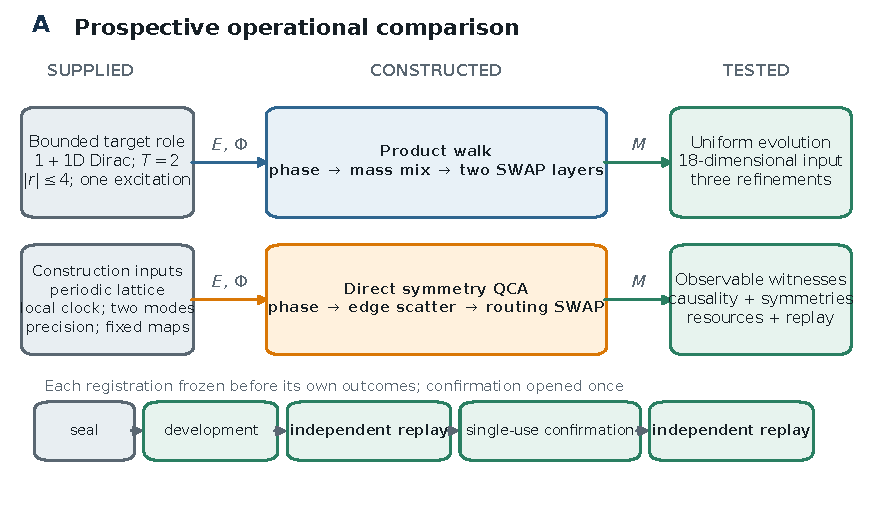
\includegraphics[width=\linewidth]{quantum_dirac_paper/figures/generated/fig01_construction_map.pdf}
  \caption{\textbf{Frozen operational-comparison contract (\conceptual).}
  The bounded target, quantum substrate, clock, constants, precision, maps,
  interventions, and gates are supplied.  The constructed objects are two
  separately registered local updates.  Both are tested with a uniform
  evolution bound, observable witnesses, structural requirements, resource
  accounting, and an algorithmically separate replay, subject to the shared
  $\pi$-reducer exception in Sec.~\ref{sec:post-result-audit}.  The arrows denote
  operational maps, not a derivation of the Dirac equation or quantum theory.}
  \label{fig:construction-map}
\end{figure}

\section{A frozen bounded Dirac operational role}
\label{sec:role}

\subsection{Target and registered domain}

In units $\hbar=c=1$, the target spinor on the periodic domain $x\in[0,L)$
obeys
\begin{equation}
  \iu\,\partial_t\psi(x,t)=H_T(t)\psi(x,t),\qquad
  H_T(t)=-\iu\sigma_z\partial_x+m(t)\sigma_x+V(x,t)I_2,
  \label{eq:target-hamiltonian}
\end{equation}
with $L=16$.  With the convention
\begin{equation}
  \psi(x)=L^{-1/2}\sum_{r\in\mathbb Z}\widehat\psi_r
  e^{\iu k_r x},\qquad k_r=2\pi r/L,
\end{equation}
the registered input sector is
\begin{equation}
  \Kin=\operatorname{span}\{\lvert r,s\rangle:-4\le r\le4,
  \ s\in\{R,L\}\}.
  \label{eq:input-sector}
\end{equation}
Thus $\dim\Kin=18$ and $|k|\le\pi/2$.  Every registered state is normalized
and supported entirely in $\Kin$.  Both registrations use physical horizon
$T=2$ and exact rational schedule boundaries.  They deliberately use
different lattice ladders and observation grids: the product walk uses
$N=256,512,1024$ and times $1/2,1,3/2,2$; the direct QCA uses
$N=320,640,1280$ and times $2/5,4/5,6/5,8/5,2$.  The distinction prevents a
failed update from inheriting the successful update's numerical
registration.

The target is finite-domain continuum Dirac evolution, not the lattice model
itself.  Potential schedules are piecewise constant in time and
formula-defined in space.  The product registration retains target Fourier
modes $|r|\le64$; the direct registration retains $|r|\le72$.  Outward analytic
tails charge the amplitude that can leave these target cutoffs.  No registered
input contains a future target trajectory.

\subsection{Fixed maps}

The role is defined by three maps held fixed within each registration
(Fig.~\ref{fig:construction-map}).  The encoding $E_N$ copies coefficients at
$r=-4,\ldots,4$ into the identically labelled normalized discrete Fourier
modes of the $N$-cell construction and zeros all other modes.  It is an
isometry; interpolation, aliasing, and outcome-dependent reconstruction are
forbidden.

The intervention map $\Phi_N$ sends the exact mass schedule and scalar
potential formula to the candidate's local gate parameters at each macrostep.
It may not alter the encoding, readout, lattice size, transport law, or error
threshold.  The product walk receives mass angle $\Delta m_q$; the direct QCA
receives $\mu_q=\Delta m_q$ and $n_q=\sqrt{1-\mu_q^2}$.  In either
registration, an active scalar potential is a separately charged leading
number phase sampled at the frozen macrostep convention.

The readout $M_N$ applies the same Born-rule harness to target and candidate.
It returns the position-grid distribution, momentum distribution, total
directional current $\langle\sigma_z\rangle$, signed local-current vector,
norm, and fidelity.  The direct protocol additionally registered an empirical
probability gate in the zone-edge sector $|q|\ge3\pi/4$; a post-result audit
found that its implemented predicate selected an empty sector, so those values
and pass flags are withdrawn (Sec.~\ref{sec:post-result-audit}).  Zitterbewegung states retain
the complete macrostep current series rather than a fitted frequency,
amplitude, or phase.

For normalized candidate and embedded target states $\psi_C$ and $\psi_T$ on
the same $N$-cell grid, define position and momentum probabilities
$p_j^{C,T}$ and $\widehat p_r^{C,T}$, local current
$j_j^{C,T}=|R_j^{C,T}|^2-|L_j^{C,T}|^2$, and total current
$J^{C,T}=\sum_j j_j^{C,T}$.  The six shared witness discrepancies are
\begin{equation}
 \begin{aligned}
 \delta_x&=\tfrac12\sum_j|p_j^C-p_j^T|,&
 \delta_k&=\tfrac12\sum_r|\widehat p_r^C-\widehat p_r^T|,\\
 \delta_J&=|J^C-J^T|,&
 \delta_j&=\sum_j|j_j^C-j_j^T|,\\
 \delta_F&=\max\{0,1-|\langle\psi_C,\psi_T\rangle|^2\},&
 \delta_Z&=\max_{t\in\mathcal O_a}|J^C(t)-J^T(t)|.
 \end{aligned}
 \label{eq:witness-metrics}
\end{equation}
Here $\mathcal O_a$ is the registered macrostep observation grid for a
Zitterbewegung scenario.  Every reported value is an outward upper enclosure
of the corresponding expression.

\subsection{Uniform comparison and witness hierarchy}

For scenario $a$, observation time $t$, and lattice size $N$, let
\begin{equation}
 D_N(a,t)=U_{C,N}[a](t)E_N-J_NU_{T,R}[a](t)P_{\mathrm{in}},
 \label{eq:discrepancy}
\end{equation}
where $P_{\mathrm{in}}$ projects onto $\Kin$, $U_{T,R}$ is the independently
constructed truncated target evolution, and $J_N$ embeds retained target
modes into the candidate grid.  Candidate amplitude outside the retained
target modes remains in the first term and therefore counts as error.  The
primary registered quantity is
\begin{equation}
 d_N(a,t)=\operatorname{upper}\!\left(\lVert D_N(a,t)\rVert_2\right)
          +\beta_{\mathrm{tail}}(a,t)+\beta_{\mathrm{num}}(a,t,N),
 \label{eq:certified-distance}
\end{equation}
an outward upper bound rather than a midpoint estimate.  Each scenario is
judged by the maximum over its registered observation times.

This uniform operator comparison is the primary gate because it applies to
every normalized input in $\Kin$, including states not explicitly plotted.
The state witnesses are nevertheless essential.  Four formula-defined state
families probe positive energy, negative energy, coherent interference, and
positive/negative-energy Zitterbewegung.  They test whether the uniform bound
translates into the registered observables and whether coherence was preserved
rather than replaced by a classical mixture.

The final layer contains structural gates that are not reducible to the
operator plot: exact radius-one causal support before wrap, attainment of both
massless cone boundaries, unitarity and numerical norm preservation, parity,
time-reversal role recovery, implementation integrity, resource accounting,
and agreement with the separate reconstruction.  The replay shared the
$\pi$-predicate defect but remains separate for the other numerical families.
The historical classifier marked a scenario as passing only if every
implemented applicable layer passed.  The later semantic audit shows why this
condition is necessary but not sufficient: an empty-set reducer can return a
passing value without implementing the specified layer.  Apart from that
disclosed exception, the hierarchy prevents a visually persuasive state
trajectory from compensating for a failed uniform, causal, or provenance
criterion.

The tested discrete symmetries are explicit.  With $\mathcal K$ denoting
componentwise complex conjugation,
\begin{equation}
 (\Pi\psi)(x_j)=\sigma_x\psi(-x_j\bmod L),\qquad
 \Theta=\sigma_x\mathcal K.
 \label{eq:tested-symmetries}
\end{equation}
For a terminal candidate map $U_a$, the parity relation is
$\Pi U_a\Pi=U_{a^\Pi}$, where $a^\Pi$ reflects the scalar potential, and the
time-reversal-role relation is
$\Theta U_a\Theta^{-1}=U_{a^{\mathrm{rev}}}^{\dagger}$, where
$a^{\mathrm{rev}}$ reverses the frozen schedule.  The registered residuals are
spectral norms of these differences restricted to the input-basis columns;
active leading potential phases may leave a prospectively gated splitting
residual rather than exact equality.

\section{Two separately registered local update realizations}
\label{sec:architectures}

Both candidates live on an oriented periodic cycle of $N$ cells with
directional labels $R$ and $L$.  Registered states occupy the global
one-excitation sector of dimension $2N$.  The direct registration declares an
explicit four-dimensional hard-core-qubit cell and full-space gates.  The
earlier product registration assigns local Hilbert dimension four and declares
ordinary transport SWAPs, but specifies its mass mixer only on the
one-excitation $R/L$ block.  Its vacuum and double-occupation phases are
therefore not frozen.  Both update laws are fully specified on the registered
one-excitation sector, but the comparison cannot use the product collision lift
to establish full-space update inequivalence.

\subsection{Ordered product walk}

The product candidate applies, from right to left,
\begin{equation}
  U_{\PW}[q]=S\,C_m[q]\,P_V[q],
  \label{eq:product-step}
\end{equation}
where
\begin{align}
  P_V[q]\lvert j,s\rangle
    &=e^{-\iu\Delta V_q(x_j)}\lvert j,s\rangle,\\
  C_m[q]
    &=e^{-\iu\Delta m_q\sigma_x},\\
  S\lvert j,R\rangle&=\lvert j+1,R\rangle,\qquad
  S\lvert j,L\rangle=\lvert j-1,L\rangle.
\end{align}
The transport $S$ is not counted as a free relabelling.  An on-site SWAP
followed by a directed edge SWAP realizes the two conditional shifts.  In the
frozen, unoptimized decomposition, a free macrostep has depth three and
gate-work $3N$; an active potential adds one leading phase layer and $N$ gates.
The free momentum block is
\begin{equation}
 U_{\PW}(k;m)=e^{-\iu\Delta k\sigma_z}e^{-\iu\Delta m\sigma_x}.
 \label{eq:product-block}
\end{equation}
Its leading global discrepancy is first order in $\Delta$, reflecting the
commutator of the ordered kinetic and mass factors
\citep{Arrighi2014DiracWalk}.

Because the product mass mixer lacks frozen $\lvert00\rangle$ and
$\lvert11\rangle$ actions, many full-space extensions share
Eq.~\eqref{eq:product-block}.  The natural hard-core extension
$\operatorname{diag}(1,e^{-\iu\Delta m\sigma_x},1)$ would carry the same
$+1$ double-occupation phase as the direct gates.  No product multiparticle or
collision-sector distinction is claimed.

\subsection{Direct symmetry-derived QCA}

For $q=k\Delta$, $\mu=m\Delta$, and $n=\sqrt{1-\mu^2}$, the established direct
one-excitation law has momentum block
\begin{equation}
 U_\mu(q)=
 \begin{pmatrix}
   ne^{-\iu q}&-\iu\mu\\
   -\iu\mu&ne^{\iu q}
 \end{pmatrix},
 \label{eq:direct-block}
\end{equation}
or real-space recurrence
\begin{equation}
 \begin{split}
 R'(x)&=nR(x-1)-\iu\mu L(x),\\
 L'(x)&=-\iu\mu R(x)+nL(x+1).
 \end{split}
 \label{eq:direct-recurrence}
\end{equation}
The law and its symmetry origin are prior art
\citep{Bisio2015QuantumFieldQCA,DAriano2014InformationPrinciples}.  What must be
declared for the present test is its finite full-space lift, circuit clock, and
collision boundary.

On edge subcells $(L_x,R_{x-1})$, in basis
$\lvert00\rangle,\lvert01\rangle,\lvert10\rangle,\lvert11\rangle$, define
\begin{equation}
 b_\mu=
 \begin{pmatrix}
 1&0&0&0\\
 0&-\iu\mu&n&0\\
 0&n&-\iu\mu&0\\
 0&0&0&1
 \end{pmatrix}.
 \label{eq:edge-gate}
\end{equation}
All disjoint edge gates form $B_\mu$; ordinary on-site SWAPs form $A$.  With
an optional leading number phase $P_V$, the physical macrostep is
\begin{equation}
  U_{\DQCA}[q]=A\,B_{\mu_q}\,P_V[q].
  \label{eq:direct-full-step}
\end{equation}
The one-excitation restriction of Eq.~\eqref{eq:direct-full-step} is exactly
Eq.~\eqref{eq:direct-recurrence}, coefficient by coefficient.  Each edge gate is
unitary because its one-excitation block is $nX-\iu\mu I$ and
$n^2+\mu^2=1$; the vacuum and double-occupation blocks are identities.  The
two partition layers are homogeneous and disjoint within a layer.  In its
frozen decomposition, one macrostep has radius one, free depth two, free
gate-work $2N$, and no ancilla.

This lift is an ordinary hard-core occupation-qubit QCA.  It fixes
$\lvert11\rangle$ with phase $+1$.  Canonical fermionic second quantization of
the same one-particle two-mode block would apply its determinant, $-1$, in the
double-occupation sector.  The two lifts agree on vacuum and one excitation
but need not agree on multiparticle scattering or spectrum
\citep{Farrelly2014CausalFermions,Mlodinow2020QFTQCA}.  The difference is an
explicit claim boundary, not a hidden implementation detail.

\subsection{Exact time-frame relation and different registered circuits}

The one-excitation blocks are algebraically close.  With
$K(q)=e^{-\iu q\sigma_z}$, the explicit half-step
$K(q)^{1/2}:=e^{-\iu q\sigma_z/2}$, and $\theta_\mu=\arcsin\mu$, the direct block obeys
\begin{equation}
 U_\mu(q)=K(q)^{1/2}e^{-\iu\theta_\mu\sigma_x}K(q)^{1/2}
 =K(q)^{-1/2}\!\left[K(q)e^{-\iu\theta_\mu\sigma_x}\right]K(q)^{1/2}.
 \label{eq:time-frame-relation}
\end{equation}
Discrete-time quantum walks admit unitarily related stroboscopic time frames,
conventionally represented by cyclic factor orderings $U'=FG$ and $U''=GF$
\citep{AsbothObuse2013TimeFrames}.  Equation~\eqref{eq:time-frame-relation}
is the model-specific instance here: the direct block is exactly a symmetric
split and is conjugate to a product-walk
block after the mass-angle remapping $\Delta m\mapsto\arcsin(m\Delta)$.  This
identity is a claim boundary, not a defect to conceal.  The conjugating factors
are chiral half-cell phases, not the integer-cell transport layers of the
registered product circuit.  The frozen specifications use different gate
partitions, intervention parameterizations, and protocol clocks.
The phrase \emph{two registered updates} therefore means two declared
one-excitation realizations under the fixed cell partition, encoding,
intervention map, and macrostep accounting.  It does not mean inequivalence
under arbitrary momentum-dependent frame changes or circuit resynthesis.

The resource difference is equally convention-bound.  In the product clock an
adjacent mass mixer and SWAP can be fused as
$X e^{-\iu\theta X}=\cos\theta\,X-\iu\sin\theta\,I$, the same
parameterized one-excitation form used by the direct edge scatter after the
time-frame change.  A library that treats arbitrary two-mode unitaries as
primitives can therefore compress
the product clock, while a SWAP-plus-rotation library would decompose the
direct scatter.  We report the sealed, nonminimal layer and gate counts because
they make the executed protocols auditable, not as compilation-invariant
complexity or a resource advantage.

On the principal small-step branch, the direct block's exact effective
generator is
\begin{equation}
 H_{\mathrm{eff}}(k,\Delta)
 =H_D(k)+\Delta^2K_2(k,m)+O(\Delta^4),
 \qquad H_D(k)=k\sigma_z+m\sigma_x,
 \label{eq:direct-effective}
\end{equation}
with
\begin{equation}
 K_2(k,m)=-\frac{m^2k}{3}\sigma_z
 +\frac{m(k^2+m^2)}{6}\sigma_x.
 \label{eq:k2}
\end{equation}
Thus one direct free step differs from $e^{-\iu\Delta H_D}$ at order
$\Delta^3$, and its global free discrepancy is second order.  Moreover,
$U_{-\Delta}(k)=U_\Delta(k)^\dagger$ exactly and
$H_{\mathrm{eff}}(k,-\Delta)=H_{\mathrm{eff}}(k,\Delta)$: the finite interaction
clock leaves an even-in-step correction without a microscopic arrow of time.
An active leading potential phase reintroduces a first-order Lie-product
contribution, which is why the direct protocol has separate direct-only and
potential-split gate families.

\begin{figure}[t]
  \centering
  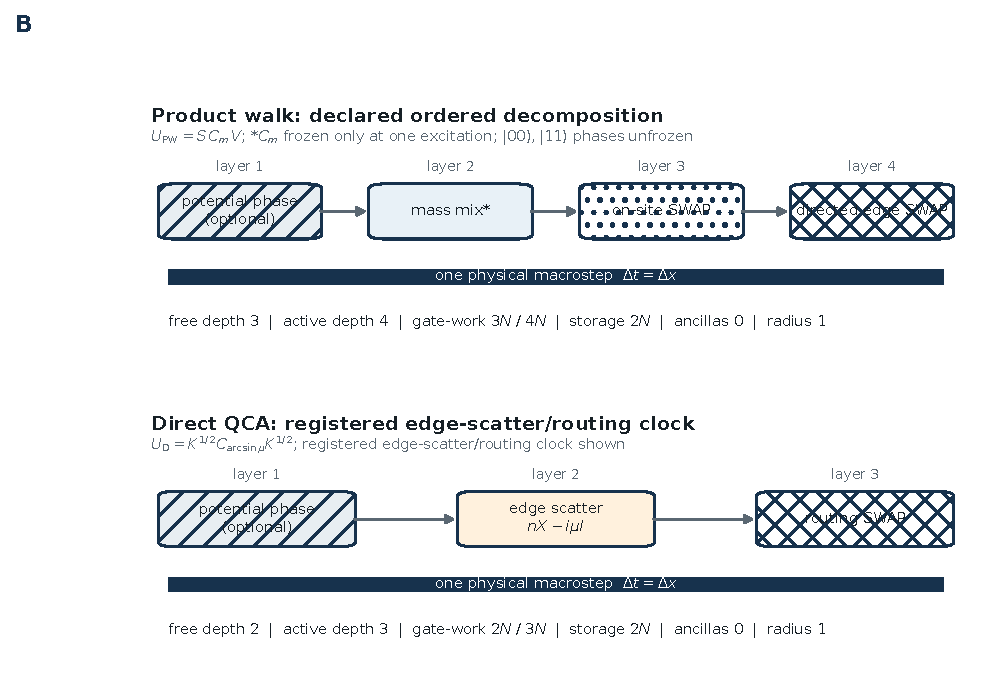
\includegraphics[width=\linewidth]{quantum_dirac_paper/figures/generated/fig02_architecture_comparison.pdf}
  \caption{\textbf{Two registered local circuits under their declared clocks
  (\analytic).}  The product walk uses a mass mixer followed by two SWAP
  transport layers.  The direct QCA uses a mass-bearing edge scatter followed
  by on-site routing.  An active scalar potential contributes one leading
  phase layer.  Counts are exact for the frozen decompositions but are
  nonminimal and change under gate fusion; they are not a hardware compilation
  or an efficiency comparison.  At one excitation the direct block is
  exactly conjugate to a mass-remapped product block by the half-cell
  time-frame change in Eq.~\eqref{eq:time-frame-relation}; the distinction shown
  here is the as-registered decomposition and clock.}
  \label{fig:architectures}
\end{figure}

\begin{table}[t]
  \centering
  \caption{Declared circuit and resource comparison.  Depth and gate-work are
  frozen protocol-clock counts, not optimized compilation minima.}
  \label{tab:architecture-comparison}
  \small
  % Generated table.
\begin{tabular}{@{}p{0.28\linewidth}p{0.32\linewidth}p{0.32\linewidth}@{}}
\toprule
Coordinate & Product walk & Direct symmetry QCA \\
\midrule
Free update & Ordered mass mix and transport & Single normalized QCA block \\
Declared localization & Mass mix; on-site and edge SWAPs & Edge scatter; on-site routing SWAP \\
Full-space scope & Mixer collision phase not frozen & Explicit hard-core $+1$ collision phase \\
Declared free / active depth & $3$ / $4$ layers & $2$ / $3$ layers \\
Declared free / active gate-work & $3N$ / $4N$ & $2N$ / $3N$ \\
Storage; ancillas & $2N$ mode labels; $0$ & $2N$ qubits; $0$ \\
Causal radius & one cell per macrostep & one cell per macrostep \\
Leading free correction & first-order global, Lie--Trotter & second-order global, symmetric time frame \\
Registered refinements & $N=256,512,1024$ & $N=320,640,1280$ \\
\bottomrule
\end{tabular}

\end{table}

\section{Prospective protocol and independent reconstruction}
\label{sec:protocol}

\subsection{Separate registrations, common logic}

The two studies share a target-domain and decision vocabulary but not a
numerical registration.  The \emph{same role} means the same continuum target,
input sector, map semantics, witness families, and causal, symmetry, and
resource categories.  Candidate law, lattice ladder, intervention cases,
numerical tolerances, and analytic convergence order are
realization-specific and were frozen separately.  A content seal binds
candidate and target code, state and scenario formulas,
maps, partitions, reducers, result schema, tests, dependencies, precision, and
stopping rule.  Registered execution remains disabled until the seal is
committed alone and identified by an annotated freeze tag.  A stage-opening
manifest is then committed alone.  The stage runs as one indivisible batch and
writes one no-clobber ledger, which is committed before inspection or replay.
Confirmation can open only if the committed development ledger passes both
its primary validator and the independent reconstruction.  This sequence is
shown at the foot of Fig.~\ref{fig:construction-map}.

The product development partition contains free light-mass, free heavy-mass,
upward mass-quench, and even-potential schedules.  Its confirmation partition
contains a downward mass quench and an odd-potential schedule.  The direct
development partition contains positive mass, negative mass, a sign-changing
quench, and a harmonic-$2$ potential.  Its confirmation partition contains a
three-stage mass pulse and a harmonic-$3$ potential.  Each partition uses four
formula-defined state families.  Product confirmation also includes a
predeclared cross-witness of its confirmation states against one development
schedule after the holdout is opened.

The confirmation schedules are single-use intervention holdouts, not draws
from a population model.  Because Eq.~\eqref{eq:certified-distance} is uniform
on $\Kin$, a finite witness-state split does not supply its logical force.  The
holdout tests whether the frozen map from a new exact intervention schedule to
the unchanged candidate continues to satisfy all uniform, observable,
structural, and replay gates.

\subsection{Frozen convergence gates}

For the product walk, every scenario must satisfy
\begin{equation}
 \begin{aligned}
 d_{256}&\le0.20,\qquad d_{512}\le0.10,\qquad d_{1024}\le0.05,\\
 d_{512}&\le0.60d_{256}+10^{-8},\qquad
 d_{1024}\le0.60d_{512}+10^{-8}.
 \end{aligned}
 \label{eq:product-absolute-gates}
\end{equation}
The scale was chosen before outcomes from the
first-order product estimate $T\Delta |km|$, with room for the registered
potential and certified tail.

The direct QCA uses its analytic finite-step signature.  Direct-only scenarios
must satisfy
\begin{equation}
 \begin{aligned}
 d_{320}&\le0.0040,\quad d_{640}\le0.0012,\quad d_{1280}\le0.0004,\\
 d_{640}&\le0.35d_{320}+10^{-10},\quad
 d_{1280}\le0.35d_{640}+10^{-10}.
 \end{aligned}
 \label{eq:direct-gates}
\end{equation}
whereas potential-split scenarios must satisfy
\begin{equation}
 \begin{aligned}
 d_{320}&\le0.020,\quad d_{640}\le0.011,\quad d_{1280}\le0.006,\\
 d_{640}&\le0.62d_{320}+10^{-10},\quad
 d_{1280}\le0.62d_{640}+10^{-10}.
 \end{aligned}
 \label{eq:potential-gates}
\end{equation}
An outcome-free 256-bit certificate bounded the complete direct one-step
remainder, telescoped it through $T=2$, charged the potential commutator,
target-cutoff tail, and numerical budget, and allowed potential-driven states
to leave the input band.  It used intermediate mode bands
$|r|\le13,17,20$ across the three refinements and charged the remaining Dyson
tail at every later step.  Its worst harmonic-$3$ envelopes were
$0.019662$, $0.007805$, and $0.002914$, below
Eq.~\eqref{eq:potential-gates}.  The certificate justified the gate scale; it did
not compute any registered trajectory, ratio, witness, or classification.

At the finest refinement, every product witness must have position and
momentum total-variation distance at most $0.05$, total- and local-current
error at most $0.10$, infidelity at most $0.0025$, and Zitterbewegung
current-series error at most $0.10$.  The corresponding direct gates are
$0.010$, $0.010$, $0.020$, $0.020$, $10^{-4}$, and $0.020$.
Both registrations require norm residual at most $10^{-12}$ and independent
state disagreement at most $10^{-11}$.  The direct potential scenarios also
specified candidate $\pi$-sector probability at most $10^{-24}$ in addition
to their analytic leakage tails; the empirical implementation of that
requirement is the exception documented in
Sec.~\ref{sec:post-result-audit}.

\subsection{Numerical and algorithmic separation}

Primary registered dynamics use \texttt{python-flint 0.9.0} Arb/Acb arithmetic
at 256 bits with outward enclosures; binary64 values are forbidden from the
registered dynamics.  The product primary evolves the candidate in real space
and the target in a retained Fourier basis.  Its independent route reconstructs
candidate gates and target evolution at 110 decimal digits with
\texttt{mpmath 1.3.0}.

For the direct update, separation is more explicit.  The primary
candidate applies the leading phase and recurrence in real space; the primary
target uses certified free blocks and spectral exponentials.  The independent
free candidate builds separate $2\times2$ momentum blocks.  Its potential
candidate constructs sparse phase, edge-scatter, and routing operators.  The
independent target rebuilds the harmonic generator and applies its exponential
through a separate high-precision route.  Candidate and verifier do not share
a candidate constructor, and target and verifier do not share a target
constructor.  This is an algorithmically separate reconstruction by the same
project, not an external replication.

\subsection{Infrastructure failures preserved rather than hidden}

The direct experiment required four separately sealed lifecycle lineages.  Version
0.1 stopped before ledger construction when the independent norm routine used
a real-symmetric eigensolver on a complex Hermitian Gram matrix.  No partial
ledger was written or inspected.  Version 0.2 wrote a primary-passing
development ledger, but replay found that a Fourier basis had been constructed
at ambient 53-bit precision before entry into the registered 256-bit context.
The certified upper bound was rigorous but failed the frozen $10^{-65}$ replay
tightness allowance.  Confirmation remained unopened.

Version 0.3 repaired precision ownership and independently reconstructed all
potential-free development scenarios, but its maximum-Gram-row-sum norm bound
became materially loose after the potential coupled registered momentum
columns.  It again stopped before confirmation.  Version 0.4 replaced only
this norm-bound reducer with a rigorous finite-precision similarity transform and
Gershgorin eigenvalue enclosure.  Approximate eigenvectors choose a basis but
carry no proof; the certified inverse, transform, and discs do.  Candidate,
target, maps, states, scenarios, partitions, thresholds, controls, and stopping
rules did not change across these infrastructure repairs.  The v0.2 and v0.3
primary classifications are not counted as verified results.  Their failure
records demonstrate why a second implementation must test certified
enclosures, not merely reproduce floating-point midpoints.

\subsection{Post-result semantic audit of the zone-edge reducer}
\label{sec:post-result-audit}

A hostile-reader audit after the v0.4 result found a shared factor-of-two error
in one reducer.  The specification defines $|q|\ge3\pi/4$ with
$q=2\pi r/N$, hence
\begin{equation}
 8|r|\ge3N.
 \label{eq:pi-sector-correct}
\end{equation}
The primary reducer, independent verifier, and non-gating rough-potential
control instead used $4|r|\ge3N$.  Since every discrete mode has
$|r|\le N/2$, that predicate selects an empty set.  All serialized empirical
$\pi$-probabilities and the rough-control value zero are therefore vacuous and
withdrawn.  The replay duplicated the predicate and is not independent evidence
for this metric.

The pre-outcome analytic leakage routine is separate and uses the correct
coarsest boundary $3N/8=120$.  Its serialized ledger values are approximately
$1.62\times10^{-261}$ for the harmonic-$2$ schedule and
$1.83\times10^{-164}$ for harmonic $3$, below the frozen $10^{-24}$ gate.
Thus the low-band leakage threshold remains supported analytically, while the
claim that its additional empirical reducer was executed correctly is
withdrawn.  No registered ledger is altered.  An audit-only recomputation of
the disclosed non-gating rough control with Eq.~\eqref{eq:pi-sector-correct}
gives $3.4860\times10^{-8}$, confirming the defect but neither repairing nor
broadening confirmation.  The serialized ledger classification field remains a
content-addressed historical fact; this manuscript reports it only with this
qualification.

\section{Registered results and post-result qualification}
\label{sec:results}

Both registrations' v0.4 development and confirmation ledgers record positive
classifications.  The
product walk passed all four development scenarios, all 16 development
witness groups, both confirmation scenarios, all eight confirmation witness
groups, and all four confirmation-state cross-witness groups.  The direct QCA
ledger classifier marked four of four development scenarios with 16 of 16
witness groups and two of two confirmation scenarios with eight of eight
witness groups as passing.  Each
committed development and confirmation ledger was accepted by the
algorithmically separate reconstruction as implemented.  The direct
$\pi$-sector predicate was later found to be empty in both primary and replay;
its measured values, associated pass flags, and one rough-potential control are withdrawn
(Sec.~\ref{sec:post-result-audit}).  The direct scenario counts are therefore
historical ledger classifications, not a claim that every intended registered
gate executed correctly.  No threshold or registered scientific input was
changed after confirmation opening.

\subsection{Certified convergence}

Figure~\ref{fig:convergence} plots every intact registered scenario-level
$d_N$ series; the withdrawn empirical $\pi$ reducer is a separate metric and
does not appear in this panel.  For the product walk, the largest certified
upper bounds across scenarios were $0.0300072572$, $0.0149954636$, and
$0.00749669028$ at $N=256,512,1024$.  The worst successive ratios were
$0.500088317$ and $0.500066986$, below the frozen $0.60$ gate.  The curves show
the registered first-order pattern without using a post-outcome slope fit as a
criterion.

For the direct QCA, the largest direct-only bounds were
$5.60191118\times10^{-4}$, $1.39960025\times10^{-4}$, and
$3.49845248\times10^{-5}$.  Their ratios lie between approximately $0.24984$
and $0.24997$, below the frozen $0.35$ gate and consistent with the analytic
second-order global discrepancy.  The largest potential-split bounds were
$2.75976665\times10^{-3}$, $1.37607978\times10^{-3}$, and
$6.87867299\times10^{-4}$, with ratios between approximately $0.49444$ and
$0.49987$, below $0.62$.  The active leading phase therefore produces the
separately anticipated first-order global family rather than being hidden
inside a direct-only convergence claim.

\begin{figure}[t]
  \centering
  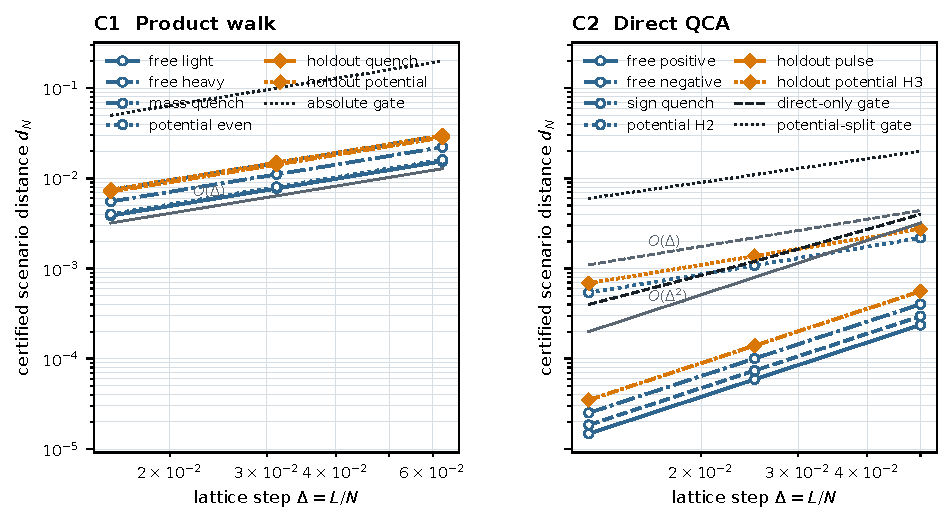
\includegraphics[width=\linewidth]{quantum_dirac_paper/figures/generated/fig03_certified_convergence.pdf}
  \caption{\textbf{Certified convergence of both frozen constructions
  (\registered).}  Each curve is the maximum over registered observation times
  of the serialized outward certified distance $d_N$ for one scenario,
  including its analytic tail and numerical budgets.
  Open markers denote development; filled diamonds denote single-use confirmation.
  The product panel retains its first-order gates; the direct panel retains
  distinct direct-only and potential-split gates.  Guide lines are analytic
  orders, not fits.  The updates have different frozen refinement and
  observation grids, and values are not normalized by their gates.}
  \label{fig:convergence}
\end{figure}

\subsection{Observable and structural witnesses}

The largest certified upper bound over development and confirmation for each
update is reported in Table~\ref{tab:witness-maxima}.  Product maxima remained
between about 11 and 249 times below their applicable gates; direct maxima
remained between about 72 and 876 times below their gates, depending on the
metric.  These margins are descriptive, not a cross-registration score: the
registrations have different steps, schedules, observation grids, and
threshold rationales.

\begin{table}[t]
  \centering
  \caption{Largest registered upper bounds for the six intact shared
  observable-witness families across both partitions.  Gates are absolute and
  were frozen separately.  The direct empirical $\pi$ value and pass flag are
  withdrawn and are not included in this table.}
  \label{tab:witness-maxima}
  \small
  % Generated table.
\begin{tabular}{@{}lrrrr@{}}
\toprule
Metric & Product max & Gate & Direct max & Gate \\
\midrule
Position TV & $0.00194047$ & $0.05$ & $9.8902\times 10^{-5}$ & $0.010$ \\
Momentum TV & $2.0061\times 10^{-4}$ & $0.05$ & $1.3971\times 10^{-4}$ & $0.010$ \\
Total-current error & $0.00844655$ & $0.10$ & $3.6737\times 10^{-5}$ & $0.020$ \\
Local-current $L_1$ & $0.00844655$ & $0.10$ & $1.9639\times 10^{-4}$ & $0.020$ \\
Infidelity & $4.5070\times 10^{-5}$ & $0.0025$ & $3.1546\times 10^{-7}$ & $0.0001$ \\
Zitterbewegung series $L_\infty$ & $0.00881467$ & $0.10$ & $2.2840\times 10^{-5}$ & $0.020$ \\
\bottomrule
\end{tabular}

\end{table}

For the product walk, the largest witness norm residual was
$3.39037\times10^{-13}$, the largest structural norm residual was
$6.22285\times10^{-13}$, and the largest parity residual was
$5.79543\times10^{-14}$, all within $10^{-12}$.  The largest fine
time-reversal-role residual was $0.0134492$ within its $0.10$ gate and passed
the first-order refinement requirement.  Exact causal support and both
massless cone boundaries passed.  The primary and independent state vectors
had serialized disagreement zero at the registered comparison precision.

For the direct QCA, the largest parity and unitarity residuals were
$9.63632\times10^{-74}$ and $1.22268\times10^{-67}$.  Potential-split
time-reversal-role residuals refined from $0.00550361$ to $0.00137599$ and
passed their $0.62$ ratio rule and $0.020$ fine gate.  All six scenarios passed
the exact implementation-integrity and causal-support gates.  The largest
analytic $\pi$-tail bound was $1.83341\times10^{-164}$, below $10^{-24}$.
The empirical $\pi$ values are not evidence because of
Eq.~\eqref{eq:pi-sector-correct}.  The largest state disagreement between
primary and independent implementations on the remaining numerical families
was $\DirectIndependentMax$, below $10^{-11}$.

\subsection{Declared resources and boundary controls}

At the finest product refinement, a free $T=2$ run uses 128 macrosteps, 384
elapsed elementary layers, and 393,216 gates.  A registered active-potential
run uses 448 layers and 458,752 gates.  At the finest direct refinement, a
free run uses 160 macrosteps, 320 layers, and 409,600 gates; the harmonic-$2$
and harmonic-$3$ potential schedules use 400 and 416 layers and 512,000 and
532,480 gates.  These totals faithfully charge each sealed protocol clock.
They are not an efficiency head-to-head because $N$, schedules, accuracy gates,
and gate-fusion conventions differ.  At equal $N$ and macrostep count, the
frozen decompositions assign free depth and work $3,3N$ to the product walk and
$2,2N$ to the direct QCA.  Section~\ref{sec:architectures} shows why these
nonminimal counts are not compilation-invariant and support no hardware or
minimal-resource advantage.

Six direct-QCA controls ran only after the confirmation primary.  Five remain
informative: the exact
opposite-mass $\pi$-partner residual was $2.49490\times10^{-111}$; a high-$q$
control had operator distance $0.00791313$; the $|\mu|=1$ endpoint had zero
maximum group velocity; a $T=12$ low-band control had distance
$0.000821366$; and the hard-core versus canonical fermionic
double-occupation phases had distance $2$.  The rough-potential zero is
withdrawn; the corrected audit-only diagnostic is $3.4860\times10^{-8}$.
These non-gating controls characterize the boundary.  They cannot repair a
failed primary and do not broaden the result.

\section{Discussion}
\label{sec:discussion}

\subsection{What the qualified two-registration evidence adds}

The central result is not that a lattice can approximate the Dirac equation.
That is known.  The intact evidence instead supports a shared core of one
bounded operational role across two sequentially tested, separately
prospective registered updates.  The product walk satisfies that core through
ordered local subdynamics; the direct QCA satisfies the same intact core
through a normalized symmetry-derived block with a different localization,
declared clock, and convergence signature, while its empirical zone-edge gate
is withdrawn.  The intact records support uniform propagator bounds, multiple
observables, and causal and symmetry constraints for both updates.
Algorithmically separate reconstruction agreed on those families while
duplicating the withdrawn $\pi$-sector predicate.  The result supports limited
robustness at the registered-specification level, not independence of the
underlying one-particle dynamics.

The coverage is only realization-level and enumerative: it covers these
two tested registered updates under the equivalence convention stated around
Eq.~\eqref{eq:time-frame-relation}.  The exact one-particle conjugacy rules out
any stronger claim that the two laws define algebraically independent
families.  ``Architecture independence'' would require a defined
architecture class and a theorem or sampling design over that class.  Nor do
the results support a primitive-class claim, because both constructions use
the same quantum substrate, periodic lattice, Born readout, and externally
specified clock and interventions.  The stronger value of the second
registration is therefore disciplined contrast, not unrestricted
generalization.

\subsection{Relation to established Dirac-QCA work}

Bisio, D'Ariano, and Tosini already derive the direct automaton, its exact
dispersion, low-mass/low-momentum Dirac regime, and a rigorous operational
comparison framed as channel discrimination
\citep{Bisio2015QuantumFieldQCA}.  They also establish Zitterbewegung and
potential scattering in the family \citep{Bisio2013DiracQCADynamics}.  Our
contribution does not supersede those results.  It embeds the established law
as the second side of a sequential two-registration study with a common role
core, realization-specific thresholds, an explicit direct-QCA full-space lift,
declared protocol clocks, precision accounting, single-use confirmation,
content-addressed ledgers, algorithmically separate reconstruction, and a
disclosed post-result defect audit.  The product full-space mass-mixer lift was
not comparably frozen.  That bounded package---not the generic idea of an
operational comparison, and not architecture-class breadth---is the novelty
claim.

\subsection{Global spectrum: a necessary boundary}

The direct QCA has exact principal band angle
\begin{equation}
 \omega(q,\mu)=\arccos\!\left(\sqrt{1-\mu^2}\cos q\right),
 \qquad q\in[-\pi,\pi).
 \label{eq:dispersion}
\end{equation}
For $0<|\mu|<1$, both the zero- and $\pi$-quasienergy circular gaps equal
$2\arcsin|\mu|$.  There is no additional zero-quasienergy cone in $1+1$
dimensions and hence no conventional low-energy doubler.  Independent
analysis of the one-dimensional Dirac quantum walk likewise finds no isolated
high-momentum/low-energy copy but does find a residual degeneracy under
simultaneous quasienergy and momentum shifts to Brillouin-zone corners,
motivating an explicit full-zone boundary even for a valid low-$q$ continuum
result \citep{Bakircioglu2025DoublingQCA}.  For
small zone-edge displacement $p$,
\begin{equation}
 U_\mu(-\pi+p)=-U_{-\mu}(p).
 \label{eq:pi-partner}
\end{equation}
After removal of the Floquet phase $-1$, the zone-edge mode has the same local
law with the opposite mass sign.  Following the distinction sharpened by
Gupta and Short \citep{Gupta2026FermionDoubling,Gupta2025DiracVacuum}, it is a
high-quasienergy pseudodoubler.  The registered low-$q$ result is not
invalidated: the input is separated from this sector, potential-generated
leakage is charged by the pre-outcome analytic bound, and the primary metric
compares propagators without asserting a global Hamiltonian logarithm.  The
intended empirical monitor is withdrawn under
Sec.~\ref{sec:post-result-audit}.  The identity
does, however, rule out a whole-zone or globally doubler-free interpretation.

At $\mu=0$, both circular gaps close and the principal logarithm becomes
branch-ambiguous at $q=-\pi$.  Accordingly, the effective-generator expansion
in Eq.~\eqref{eq:direct-effective} is confined to a branch-safe neighborhood of
$q=0$.  This reconciles a bounded continuum role with the global Floquet
spectrum and makes the limitation visible rather than relegating it to an
unmonitored high-momentum sector.

\begin{figure}[t]
  \centering
  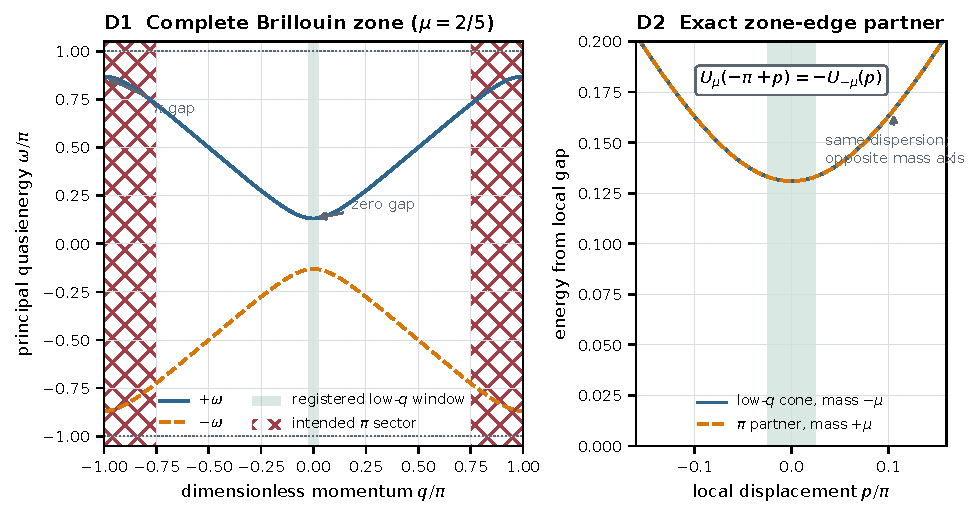
\includegraphics[width=\linewidth]{quantum_dirac_paper/figures/generated/fig04_spectrum_domain.pdf}
  \caption{\textbf{Global spectrum and bounded claim domain (\analytic; not a
  registered outcome).}  For the disclosed illustrative value $\mu=2/5$, the
  bands follow Eq.~\eqref{eq:dispersion}.  The central strip is the coarsest
  registered input window $|q|\le\pi/40$; finer windows are narrower.  Hatching
  marks the intended $\pi$ sector $|q|\ge3\pi/4$ used by the valid analytic
  tail; the empirical reducer for that sector is withdrawn.  The exact
  zone-edge identity exposes a high-quasienergy opposite-mass pseudodoubler.}
  \label{fig:spectrum}
\end{figure}

\subsection{Full-space lift and further tests}

The hard-core/fermionic collision-phase difference is not visible to any
one-excitation witness.  It becomes material under second quantization,
collisions, interactions, or a filled sea.  Published causal fermionic and
multiparticle QCA constructions show that those extensions require additional
structure \citep{Farrelly2014CausalFermions,Mlodinow2020QFTQCA}.  They cannot be
inferred from the present pass.  A canonical fermionic or interacting follow-on
should therefore receive a new search identifier, global-spectrum audit,
vacuum definition, and prospective protocol.

The direct hard-core lift is explicit, but the product registration does not
fix its mass mixer's vacuum and double-occupation phases.  The present
one-excitation comparison therefore supplies no product-versus-direct
collision claim.  A follow-on that uses full-space behavior must freeze both
lifts symmetrically.

The same separation applies to a differently localized circuit or a classical
reversible lattice gas.  A nominal Strang split is not automatically a third
case because Eq.~\eqref{eq:time-frame-relation} already exposes an exact
symmetric factorization of the direct block.  A genuinely new case would need
a predeclared circuit-equivalence criterion.  Either direction could increase
breadth, but neither
changes the interpretation of the completed two-registration result.  New
science should begin only after this manuscript's claims and limitations are
stable, under a separately registered search rather than as post-outcome
robustness tuning.

\begin{figure}[t]
  \centering
  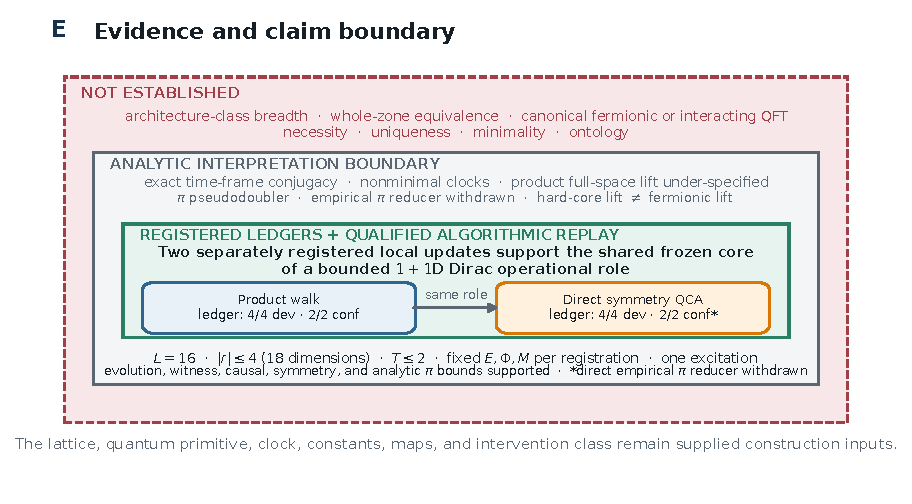
\includegraphics[width=\linewidth]{quantum_dirac_paper/figures/generated/fig05_claim_boundary.pdf}
  \caption{\textbf{Evidence and claim boundary (\conceptual{} synthesis).}
  The inner domain is the qualified registered result.  The middle domain contains
  analytic constraints required to interpret it.  The outer field lists
  claims not established.  Inclusion denotes logical scope, not evidential
  probability.  The withdrawn empirical $\pi$ reducer is shown as an audit
  boundary rather than positive evidence.}
  \label{fig:claim-boundary}
\end{figure}

\section{Limitations and claim discipline}
\label{sec:limitations}

The result is deliberately bounded in several independent directions.

\paragraph{Finite physical domain.}
The target role covers $L=16$, $T\le2$, exact registered mass and scalar
potential schedules, input modes $|r|\le4$, and three refinements per
update.  It does not establish all-scale continuum equivalence,
nonperiodic boundaries, arbitrary interventions, vector or gauge potentials,
curved geometry, feedback, or long-time uniformity.  Three refinements can
test frozen ratio gates but cannot by themselves establish an unrestricted
asymptotic theorem.

\paragraph{Single-excitation sector.}
All primary maps and outcomes concern one excitation.  The direct circuit is
unitary on the complete hard-core qubit Hilbert space, but its collision phase
is not a canonical fermionic lift.  Its empty hard-core vacuum is fixed, but
no physically identified fermionic vacuum or Dirac sea, free-fermion field,
multiparticle scattering, interaction, or particle creation is demonstrated.

\paragraph{Two registered updates, not an inequivalent architecture class.}
The qualified comparison covers a product walk and one direct QCA as registered
one-excitation update specifications.  Their
one-excitation blocks are exactly related by the half-cell time-frame conjugacy
in Eq.~\eqref{eq:time-frame-relation}, and their declared resource difference
can be removed or reversed by changing the gate-fusion library.  The product
mass mixer's full-space collision phase was not frozen.  The demonstrated
difference is therefore only between the as-registered gate partitions,
intervention parameterizations, and protocol clocks.  The updates also share a
quantum primitive, oriented cycle, Born readout, and externally specified
clock.  No equivalence class or distribution over architectures was defined,
so there is no claim of architecture independence.

\paragraph{Constructive sufficiency only.}
The target Hamiltonian, lattice, quantum substrate, clock, constants,
precision, maps, and intervention class are supplied construction inputs.
The intact pass evidence shows that the declared local mechanisms are
sufficient within the role.
It does not show that they are necessary, unique, minimal, ontologically
fundamental, or derivable from information alone.  It also says nothing about
a finite-classical-bit realization.

\paragraph{Verification independence.}
The replay uses a separately implemented numerical route with different
candidate and target constructors and higher precision.  It was produced by
the same project and shares the frozen mathematical specification.  We
therefore call it algorithmically separate reconstruction or replay, not an
external replication.  A third-party clean-room reproduction remains
valuable.  The post-result audit also shows a limit of algorithmic separation:
both implementations copied the same erroneous $\pi$-sector predicate, so
replay is not semantic specification diversity.

\paragraph{Thresholds and record granularity.}
Absolute and ratio gates were analytically motivated and frozen, but any
finite threshold encodes a chosen accuracy standard.  Passing it is not exact
continuum equality.  Product ledgers serialize per-time non-Zitterbewegung
witness observations; direct ledgers serialize their maxima and the full
Zitterbewegung current series.  The direct uniform operator records retain all
five observation upper bounds, but their times are joined by canonical index
to the target specification.  This asymmetry does not affect registered
maxima or classifications, but it prevents a perfectly symmetric
per-time supplemental witness table.

\paragraph{Withdrawn empirical leakage reducer.}
The direct empirical $\pi$-sector reducer and rough-potential control are
invalid because their predicate selects no modes.  The pre-outcome analytic
tail uses the correct boundary and remains below its frozen threshold, but the
paper does not count the empirical zero or its duplicated replay as positive
evidence.  Corrected registered measurement would require a separately opened
follow-on.

Figure~\ref{fig:claim-boundary} summarizes these exclusions.  They are not generic
disclaimers: analytic leakage accounting, the mass endpoint, long horizon,
global spectrum, and collision-phase control make several of them executable
failure boundaries.  The withdrawn reducer demonstrates why semantic audits
must complement byte-level replay.

\section{Conclusion}
\label{sec:conclusion}

Two separately prospective registrations tested an ordered product walk and
the established direct Dirac QCA against a common, bounded, low-momentum
single-excitation role.  All four counted v0.4 stage ledgers recorded positive
classifications, and an algorithmically separate implementation reconstructed
the committed computations.  The intact evidence supports qualified
constructive sufficiency for the shared role core: uniform evolution bounds,
observable witnesses, causal and symmetry requirements, and the correctly
derived analytic zone-edge bound.  It does not support the complete originally
registered direct role, because the empirical zone-edge reducer and its pass
flags are withdrawn.

The exact time-frame conjugacy also changes the interpretation of the second
registration.  It provides disciplined, separately frozen coverage of two
declared update specifications and protocol clocks, not breadth across proven
inequivalent architecture classes or a compilation-invariant resource
advantage.  The durable contribution is therefore the combination of an
executable operational role, prospective stage separation, explicit locality
and resource accounting, content-addressed evidence, algorithmically separate
reconstruction, and an audit trail that preserves rather than conceals a
post-result defect.  Any genuinely broader architecture or corrected empirical
zone-edge test belongs in a separately registered follow-on.

\section{Reproducibility and content-addressed provenance}
\label{sec:reproducibility}

All plotted registered-result values and generated result tables derive from
the four counted v0.4 JSON stage ledgers.  The figure and table generator refuses to run if
any ledger or registered specification hash differs from its recorded SHA-256.
It parses serialized outward upper values, preserves scenario order, generates
vector PDF and inspection PNG assets, and writes a sidecar manifest containing
input, analytic-source, generator, and output hashes, tool versions, and the
evidence class of every figure.  No registered number is manually transcribed
into a plot.  Prose summaries are human-readable transcriptions and should be
checked against the generated tables and ledgers.

The product history is linear from freeze commit \texttt{d942c114} through
development opening \texttt{cfaaabe9}, development result
\texttt{e5a5c4e9}, confirmation opening \texttt{0181ce0f}, confirmation result
\texttt{c7e9a216}, and verified documentation \texttt{490dab6b}.  The direct
v0.4 history is linear from freeze \texttt{890962df} through development
opening \texttt{f5f5d604}, development result \texttt{b96e70a1}, confirmation
opening \texttt{6398124a}, and confirmation result \texttt{0795a6ef}.  Each
freeze, opening, and result commit introduces exactly its one registered
artifact.  Earlier direct lineages remain content-addressed and are not counted
as positive evidence.

The complete local build is
\begin{verbatim}
make quantum-dirac-paper
\end{verbatim}
which verifies ledger hashes, regenerates derived tables and all five figures,
reproduces the post-result $\pi$-sector audit, runs the archived-result
validator, and compiles this manuscript with \texttt{latexmk}.  A full
expensive reconstruction can be run separately through the
checkpoint-specific direct-QCA verification commands documented with the
result.  The
registered primary environment records \texttt{python-flint 0.9.0}, 256-bit
Arb/Acb precision, and outward ball enclosures.  The replay records
\texttt{mpmath 1.3.0} at 110 decimal digits.  The manuscript plotting layer
uses pinned NumPy and Matplotlib versions only after ledger validation; it is
not part of the scientific evaluator.

The generated provenance manifest is
\texttt{quantum\_dirac\_paper/generated/figure\_manifest.json}.  Human-readable
terminal summaries sit beside each experiment.  The direct result summary
also records the stage-specific replay receipt, ledger hashes, seal hash,
freeze and result commits, terminal classification, the known shared
$\pi$-predicate exception, and non-gating boundary controls.  The receipt
certifies reproduction of the implemented checkpoint bytes; it does not cure
or independently validate the withdrawn predicate.

\begin{table}[t]
  \centering
  \caption{Content-addressed registered ledgers.  The direct-QCA positive
  classifications are historical ledger fields qualified by the withdrawn
  empirical $\pi$-sector reducer.  Full hashes are recorded in the generated
  manifest and experiment result summaries.}
  \label{tab:provenance}
  \small
  % Generated table.
\begin{tabular}{@{}llll@{}}
\toprule
Architecture & Partition & Classification & Ledger SHA-256 \\
\midrule
Product walk & Development & \texttt{development\_passed} & \texttt{c9f445358a7a\ldots} \\
Product walk & Confirmation & \texttt{constructive\_sufficiency\_passed\_frozen\_dirac\_sector} & \texttt{34c16fd95914\ldots} \\
Direct QCA & Development & \texttt{development\_passed} & \texttt{89d7c65a37bf\ldots} \\
Direct QCA & Confirmation & \texttt{constructive\_sufficiency\_passed\_direct\_symmetry\_qca\_sector} & \texttt{be5a9f85770e\ldots} \\
\bottomrule
\end{tabular}

\end{table}

The complete ledger SHA-256 values are recorded in the generated manifest and
the two experiment result summaries; Table~\ref{tab:provenance} prints
unambiguous prefixes for reading.  The hashes make local evidence
tamper-evident; absent an external timestamped deposit they are not themselves
an archival guarantee, and they do not replace independent scientific review.
The final PDF hash and build-tool versions are written beside the deliverable
in \texttt{output/pdf}.

\appendix

\section{Scenario-level certified distances}
\label{app:scenario-distances}

Table~\ref{tab:scenario-distances} gives every scenario maximum used in
Fig.~\ref{fig:convergence}.  Values are the serialized outward endpoints of the
certified bounds.  ``Coarse,'' ``middle,'' and ``fine'' denote
$N=256,512,1024$ for the product walk and $N=320,640,1280$ for the direct QCA.

\begin{table}[htbp]
  \centering
  \caption{All registered scenario-level certified-distance upper bounds.}
  \label{tab:scenario-distances}
  \small
  % Generated table.
\begin{tabular}{@{}llrrr@{}}
\toprule
Architecture / partition & Scenario & Coarse & Middle & Fine \\
\midrule
Product walk / development & free light & $0.0154366$ & $0.00771499$ & $0.00385708$ \\
Product walk / development & free heavy & $0.0297087$ & $0.0148466$ & $0.00742234$ \\
Product walk / development & mass quench & $0.0221470$ & $0.0110755$ & $0.00553848$ \\
Product walk / development & potential even & $0.0160532$ & $0.00802447$ & $0.00401181$ \\
Product walk / confirmation & holdout quench & $0.0284341$ & $0.0142083$ & $0.00710284$ \\
Product walk / confirmation & holdout potential & $0.0300073$ & $0.0149955$ & $0.00749669$ \\
Direct QCA / development & free positive & $2.3676\times 10^{-4}$ & $5.9158\times 10^{-5}$ & $1.4787\times 10^{-5}$ \\
Direct QCA / development & free negative & $2.9634\times 10^{-4}$ & $7.4045\times 10^{-5}$ & $1.8509\times 10^{-5}$ \\
Direct QCA / development & sign quench & $4.0285\times 10^{-4}$ & $1.0066\times 10^{-4}$ & $2.5161\times 10^{-5}$ \\
Direct QCA / development & potential H2 & $0.00218949$ & $0.00108256$ & $5.3983\times 10^{-4}$ \\
Direct QCA / confirmation & holdout pulse & $5.6019\times 10^{-4}$ & $1.3996\times 10^{-4}$ & $3.4985\times 10^{-5}$ \\
Direct QCA / confirmation & holdout potential H3 & $0.00275977$ & $0.00137608$ & $6.8787\times 10^{-4}$ \\
\bottomrule
\end{tabular}

\end{table}

\section{Frozen schedules and formula-defined state witnesses}
\label{app:registered-inputs}

The manuscript generator verifies the SHA-256 digest of each update
registration's frozen scenario and state specification before emitting these tables.  Write
$[t_0,t_1)$ for a schedule interval.  The registered mass is piecewise
constant, $m(t)=m_j$ on its listed interval, and the potential entries mean
\begin{equation}
  V(x,t)=a_j\cos\!\left(2\pi h_j x/L+\phi_j\right),
  \qquad t\in[t_{0,j},t_{1,j}),
  \label{eq:registered-potential}
\end{equation}
with $V=0$ outside all listed intervals.  The product-walk specification has
$h_j=1$ throughout.  Table~\ref{tab:registered-scenarios} is therefore an
exact compact transcription, not a fit to the result ledgers.

\begin{table}[htbp]
  \centering
  \caption{Exact frozen mass and potential schedules.  PW denotes the product
  walk; DQCA denotes the direct symmetry QCA.}
  \label{tab:registered-scenarios}
  \scriptsize
  \setlength{\tabcolsep}{3pt}
  % Generated from four hash-verified frozen specification files.
\begin{tabularx}{\linewidth}{@{}p{0.10\linewidth}p{0.29\linewidth}X X@{}}
\toprule
Update / split & Registered scenario & $m$: value and interval & $V$: $(h,a,\phi;[t_0,t_1))$ \\
\midrule
PW / dev. & \texttt{DEV-\allowbreak{}FREE-\allowbreak{}LIGHT} & $\tfrac{1}{4}\;[0,2)$ & $0$ \\
PW / dev. & \texttt{DEV-\allowbreak{}FREE-\allowbreak{}HEAVY} & $\tfrac{1}{2}\;[0,2)$ & $0$ \\
PW / dev. & \texttt{DEV-\allowbreak{}QUENCH-\allowbreak{}UP} & $\tfrac{1}{4}\;[0,1);\;\tfrac{1}{2}\;[1,2)$ & $0$ \\
PW / dev. & \texttt{DEV-\allowbreak{}POTENTIAL-\allowbreak{}EVEN} & $\tfrac{1}{4}\;[0,2)$ & $(1,\tfrac{1}{4},0;[\tfrac{1}{2},\tfrac{3}{2}))$ \\
PW / conf. & \texttt{HOLDOUT-\allowbreak{}QUENCH-\allowbreak{}DOWN} & $\tfrac{1}{2}\;[0,\tfrac{3}{4});\;\tfrac{1}{4}\;[\tfrac{3}{4},2)$ & $0$ \\
PW / conf. & \texttt{HOLDOUT-\allowbreak{}POTENTIAL-\allowbreak{}ODD} & $\tfrac{1}{2}\;[0,2)$ & $(1,\tfrac{1}{4},\tfrac{\pi}{2};[\tfrac{1}{4},\tfrac{5}{4}))$ \\
DQCA / dev. & \texttt{DEV-\allowbreak{}DIRECT-\allowbreak{}FREE-\allowbreak{}POS} & $\tfrac{1}{3}\;[0,2)$ & $0$ \\
DQCA / dev. & \texttt{DEV-\allowbreak{}DIRECT-\allowbreak{}FREE-\allowbreak{}NEG} & $-\tfrac{2}{5}\;[0,2)$ & $0$ \\
DQCA / dev. & \texttt{DEV-\allowbreak{}DIRECT-\allowbreak{}SIGN-\allowbreak{}QUENCH} & $\tfrac{1}{4}\;[0,\tfrac{4}{5});\;-\tfrac{1}{3}\;[\tfrac{4}{5},2)$ & $0$ \\
DQCA / dev. & \texttt{DEV-\allowbreak{}DIRECT-\allowbreak{}POTENTIAL-\allowbreak{}H2} & $\tfrac{2}{5}\;[0,2)$ & $(2,\tfrac{1}{8},0;[\tfrac{3}{10},\tfrac{13}{10}))$ \\
DQCA / conf. & \texttt{HOLDOUT-\allowbreak{}DIRECT-\allowbreak{}MASS-\allowbreak{}PULSE} & $-\tfrac{1}{5}\;[0,\tfrac{7}{20});\;\tfrac{3}{5}\;[\tfrac{7}{20},\tfrac{27}{20});\;\tfrac{1}{5}\;[\tfrac{27}{20},2)$ & $0$ \\
DQCA / conf. & \texttt{HOLDOUT-\allowbreak{}DIRECT-\allowbreak{}POTENTIAL-\allowbreak{}H3} & $-\tfrac{1}{3}\;[0,2)$ & $(3,\tfrac{1}{10},\tfrac{\pi}{2};[\tfrac{1}{4},\tfrac{29}{20}))$ \\
\bottomrule
\end{tabularx}

\end{table}

Every state was generated from parameters rather than stored amplitudes.  Let
$\mathsf N[v]=v/\lVert v\rVert_2$.  For $p=(r_0,w,x_0)$,
$k_r=2\pi r/L$, and $r=-4,\ldots,4$, first form the raw spinor-valued packet
and then normalize that packet individually:
\begin{align}
 g_s(r;p,m_0)
   &=e^{-(r-r_0)^2/(2w^2)}e^{-\iu k_rx_0}\chi_s(k_r;m_0),\\
 \psi_s(p;m_0)&=\mathsf N[g_s(\,\cdot\,;p,m_0)],
 \qquad s\in\{+,-\}.
 \label{eq:registered-packet}
\end{align}
Here $\chi_s$ is the normalized $s$-energy eigenvector of
$k_r\sigma_z+m_0\sigma_x$, fixed by taking its first nonzero component real
and positive, and $m_0=m(0)$ for the scenario.  Positive and negative states
use $s=+$ and $s=-$, respectively.  The implementation then normalizes each
composite separately after combining already normalized packets:
\begin{align}
 \psi_{\mathrm{int}}(p_1,p_2,\phi;m_0)
   &=\mathsf N\!\left[\psi_+(p_1;m_0)+e^{\iu\phi}\psi_+(p_2;m_0)\right],\\
 \psi_{\mathrm Z}(p,\phi;m_0)
   &=\mathsf N\!\left[\psi_+(p;m_0)+e^{\iu\phi}\psi_-(p;m_0)\right].
 \label{eq:registered-composite-states}
\end{align}
Table~\ref{tab:registered-states} records every exact parameter tuple.  For
interference rows, $p_1$ and $p_2$ are packet tuples; for all other rows,
$p=(r_0,w,x_0)$.

\begin{table}[htbp]
  \centering
  \caption{Exact frozen formula parameters for all state witnesses.}
  \label{tab:registered-states}
  \scriptsize
  \setlength{\tabcolsep}{3pt}
  % Generated from four hash-verified frozen specification files.
\begin{tabularx}{\linewidth}{@{}p{0.10\linewidth}p{0.32\linewidth}p{0.19\linewidth}X@{}}
\toprule
Update / split & Registered state & Type & Exact parameters \\
\midrule
PW / dev. & \texttt{DEV-\allowbreak{}STATE-\allowbreak{}POS} & positive energy & $p=(2,1,4)$ \\
PW / dev. & \texttt{DEV-\allowbreak{}STATE-\allowbreak{}NEG} & negative energy & $p=(-2,1,12)$ \\
PW / dev. & \texttt{DEV-\allowbreak{}STATE-\allowbreak{}INTERFERENCE} & positive interference & $p_1=(2,1,4);\ p_2=(-2,1,12);\ \phi=\tfrac{\pi}{2}$ \\
PW / dev. & \texttt{DEV-\allowbreak{}STATE-\allowbreak{}ZITTER} & energy mixture & $p=(1,1,8);\ \phi=\tfrac{\pi}{3}$ \\
PW / conf. & \texttt{HOLDOUT-\allowbreak{}STATE-\allowbreak{}POS} & positive energy & $p=(-1,\tfrac{3}{4},6)$ \\
PW / conf. & \texttt{HOLDOUT-\allowbreak{}STATE-\allowbreak{}NEG} & negative energy & $p=(3,\tfrac{3}{4},10)$ \\
PW / conf. & \texttt{HOLDOUT-\allowbreak{}STATE-\allowbreak{}INTERFERENCE} & positive interference & $p_1=(1,\tfrac{3}{4},2);\ p_2=(-3,\tfrac{3}{4},9);\ \phi=\tfrac{\pi}{5}$ \\
PW / conf. & \texttt{HOLDOUT-\allowbreak{}STATE-\allowbreak{}ZITTER} & energy mixture & $p=(-2,\tfrac{3}{4},3);\ \phi=-\tfrac{\pi}{4}$ \\
DQCA / dev. & \texttt{DEV-\allowbreak{}DIRECT-\allowbreak{}STATE-\allowbreak{}POS} & positive energy & $p=(\tfrac{3}{2},\tfrac{5}{6},3)$ \\
DQCA / dev. & \texttt{DEV-\allowbreak{}DIRECT-\allowbreak{}STATE-\allowbreak{}NEG} & negative energy & $p=(-\tfrac{5}{2},\tfrac{2}{3},11)$ \\
DQCA / dev. & \texttt{DEV-\allowbreak{}DIRECT-\allowbreak{}STATE-\allowbreak{}INTERFERENCE} & positive interference & $p_1=(\tfrac{5}{2},\tfrac{4}{5},2);\ p_2=(-\tfrac{3}{2},\tfrac{4}{5},13);\ \phi=\tfrac{2\pi}{7}$ \\
DQCA / dev. & \texttt{DEV-\allowbreak{}DIRECT-\allowbreak{}STATE-\allowbreak{}ZITTER} & energy mixture & $p=(\tfrac{1}{2},\tfrac{4}{5},7);\ \phi=\tfrac{2\pi}{5}$ \\
DQCA / conf. & \texttt{HOLDOUT-\allowbreak{}DIRECT-\allowbreak{}STATE-\allowbreak{}POS} & positive energy & $p=(-\tfrac{3}{2},\tfrac{7}{10},5)$ \\
DQCA / conf. & \texttt{HOLDOUT-\allowbreak{}DIRECT-\allowbreak{}STATE-\allowbreak{}NEG} & negative energy & $p=(\tfrac{5}{2},\tfrac{7}{10},13)$ \\
DQCA / conf. & \texttt{HOLDOUT-\allowbreak{}DIRECT-\allowbreak{}STATE-\allowbreak{}INTERFERENCE} & positive interference & $p_1=(\tfrac{1}{2},\tfrac{3}{4},1);\ p_2=(-\tfrac{5}{2},\tfrac{3}{4},10);\ \phi=-\tfrac{\pi}{6}$ \\
DQCA / conf. & \texttt{HOLDOUT-\allowbreak{}DIRECT-\allowbreak{}STATE-\allowbreak{}ZITTER} & energy mixture & $p=(-\tfrac{1}{2},\tfrac{3}{4},4);\ \phi=\tfrac{3\pi}{7}$ \\
\bottomrule
\end{tabularx}

\end{table}

\section{Analytic structure and exact boundaries}

For the direct free block, write
\begin{equation}
 U_\Delta(k)=aI-\iu(b_x\sigma_x+b_z\sigma_z),\qquad
 \mu=m\Delta,\quad n=\sqrt{1-\mu^2},\quad
 a=n\cos(k\Delta),\quad b_x=\mu,\quad b_z=n\sin(k\Delta).
\end{equation}
Let $\rho=\sqrt{b_x^2+b_z^2}$ and
$\omega=\operatorname{atan2}(\rho,a)$ on the principal branch.  Because
$a^2+\rho^2=1$, the principal effective generator is exactly
$H_{\mathrm{eff}}=\frac{\omega}{\Delta\rho}
(b_x\sigma_x+b_z\sigma_z)$, with its continuous $\rho\to0$, $a\to+1$ value
understood in the registered branch-safe neighborhood of the identity.
Expanding $\omega/\rho$ and the two
axis components gives Eqs.~\eqref{eq:direct-effective} and \eqref{eq:k2}.  An independent matrix-log
fixture reconstructs the same generator from a power series without calling
the axis--angle implementation.  Halving $\Delta$ produces the predeclared
$1/16$ corrected-generator residual ratio and $1/8$ one-step propagator ratio
on disclosed nonregistered fixtures.

The global direct spectrum follows from
\begin{equation}
 \det U_\mu(q)=1,\qquad \operatorname{tr}U_\mu(q)=2n\cos q.
\end{equation}
For $0<|\mu|<1$, group velocity obeys
\begin{equation}
 |v(q)|\le n=\sqrt{1-\mu^2}\le1,
\end{equation}
consistent with radius-one causal support.  At $|\mu|=1$ the bands are flat at
$\pm\pi/2$ and group velocity is zero.  For $|\mu|>1$, $n$ is imaginary and
the displayed family is not unitary.  The registered direct margin
$|\mu|\le3/100$ at the coarsest step is therefore strict.

The exact hard-core collision choice appears in Eq.~\eqref{eq:edge-gate}.  For a
number-preserving one-particle unitary $V$, canonical fermionic second
quantization acts on double occupation by $\det V$.  Both the edge-scatter
one-particle block and the routing SWAP have determinant $-1$, while the
declared qubit gates use phase $+1$.  This algebraic distance of $2$ is the
post-primary collision control reported in Sec.~\ref{sec:results}.

\section{Interpretation of confirmation}

The primary comparison is a deterministic, certified statement uniform over
the finite input sector.  Consequently, the confirmation partition does not
estimate a frequentist population effect.  Its evidential role is procedural
and interventional: exact schedules and state formulas unused in update
construction or development assessment are opened once, propagated by the sealed code, and required to
pass without replacing any map, threshold, or candidate byte.  Reporting
scenario and witness counts should therefore not be read as a sample-size
claim.  The correctly implemented members of the registered finite test suite
passed, and the evolution certificate covers every normalized state in $\Kin$
for those scenarios.  The empirical $\pi$-sector member is excluded from that
sentence because its empty-set reducer is withdrawn under
Sec.~\ref{sec:post-result-audit}.


\bibliographystyle{unsrtnat}
\bibliography{quantum_dirac_paper/bibliography}

\end{document}
